\documentclass[11pt, oneside, a4paper]{article}
\usepackage{ifpdf}
\usepackage{graphicx}
\usepackage[colorlinks,bookmarksopen,linkcolor=black,pdfauthor={Vikram},urlcolor=blue]{hyperref}
\usepackage[colorlinks,bookmarksopen]{hyperref}
\usepackage[hmargin=1.5cm,vmargin=2.5cm]{geometry}
\usepackage{algorithmic}
\usepackage{algorithm}
\begin{document}
\begin{center}
\textbf{VISVESWARAYA TECHNOLOGICAL UNIVERSITY}
\end{center}
\begin{center}
\textbf{BELGAUM}\\
\thispagestyle{empty}
\begin{figure}[htb]
\begin{center}
\ifpdf

\includegraphics[scale=0.50]{vtu.png}
\else
\fi
\end{center}
\end{figure}
\textbf{SRI JAYACHAMARAJENDRA COLLEGE OF ENGINEERING,}
\textbf{MYSORE-570006}\\
\textsc{department of computer science and engineering}
\end{center}
\begin{figure}[htb]
\begin{center}
\ifpdf

\includegraphics[scale=0.30]{./logo.png}
\else
\fi
\end{center}
\end{figure}
\begin{center}
\textbf{\underline{Report on}}\\
\textsc{\\IMPLEMENTATION OF RED-BLACK TREE\\}
\emph{\\Guidance of}\\
\textbf{\\N.R. PRASHANTH}\\
\textit{Professor}\\
\textit{Department of CS$\&$E, SJCE, Mysore.}\\
\vspace{1in}
\textbf{\underline{Done By:}}\\
\textsc{\\VIKRAM T.V.}\\
4th Semester,\\ Computer Science and Engineering,\\
S.J.C.E, Mysore\\
\title {IMPLEMENTATION OF RED-BLACK TREE\\}
\end{center}
\newpage
\thispagestyle{empty}
\tableofcontents
\newpage
\pagenumbering{arabic}

\twocolumn
\section{Introduction}
Red black tree, a variant of binary tree, is determined by the color assigned to each of the node.  The color may be either 'red' or 'black'.  Knowing the color of a node helps us to balance the tree.

\section{Properties and Rotation}
A binary tree is said to be a red black tree if it satisfies the following properties.
\begin{itemize}
\item Every node is either red or black.
\item The root is black.
\item Every null leaf is black.
\item If a node is red, then both its children are black.
\item For each node, all paths from the node to descendant leaves contain the same number of black nodes (known as 'black height').
\end{itemize}

In order to balance the tree using the color properties, we may need to change color of the nodes and adjust the pointers.  Adjusting pointers is done by \textbf {rotation}, which prevents the binary search property of the tree.  There are two kinds of rotation - left rotation and right rotation.  Consider a tree with internal nodes 'x' and 'y' and 'A', 'B', 'C' as leaf nodes.  The left and right rotations are complementary and are as shown in the figure.
\begin{figure}[htb]
\begin{center}
\ifpdf
	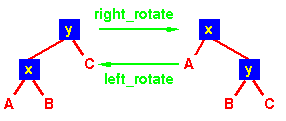
\includegraphics[scale=0.50]{rbtRotate.png}
\else
\fi
\caption{Rotation of a tree}
\label{fig:Rotation}
\end{center}
\end{figure}

\section{The Algorithm}
The algorithm for insertion and deletion involves coloring and rotation to preserve the red black properties of the tree.
\subsection{Insertion}
Insertion of a new node to the tree involves two stages.  First, the new node 'z' is colored 'red' and inserted as if it were an ordinary binary search tree.  Next, the rotations are done to 'fixup' the insertion and can be one of the following cases:
\begin{itemize}
\item Case 1: Uncle[z] is also 'red'.\\
	In this case, both parent[z] and uncle[z] are colored 'black' and grandparent[z] is colored 'red'.  Finally assign 'z' to its grandparent.
\item Case 2: Uncle[z] is 'black'.\\
	Case 2a: If parent[z] is left child of its parent and 'z' is a \emph {right child} of its parent, then left rotate at parent[z] (and perform case 3).\\Case 2b: if parent[z] is right child of its parent and 'z' is a \emph {left child} of its parent, then right rotate at parent[z] (and perform case 3).\\  These operations have not changed any colors.
\item Case 3: Uncle[z] is again 'black', but may have resulted from case 2 after rotation.\\
	Assign parent[z] with 'black', grandParent[z] with 'red' and perform right rotation for case 2a or left rotation for case 2b at grandParent[z].
\end{itemize}
Perform the above cases until parent[z] remains 'red'.  Finally, assign the color[T] as 'black'.\\\\
The above cases are represented by the following algorithm; where color of node 'z' is represented as color[z], left and right children as left[z] and right[z] repectively.

\begin{algorithm}
\caption {RBT Insert}
\label {alg1}
\begin{algorithmic}[1]
\STATE \textbf {rbtInsert (T, z)}
\STATE insert node 'z' as if it were inserted to an ordinary binary search tree.
\STATE color[z] $\leftarrow$ RED
\STATE rbtInsertFixup (T, z)
\end{algorithmic}
\end{algorithm}

\begin{algorithm}
\caption {RBT Insert Fixup}
\label {alg2}
\begin{algorithmic}[1]
\STATE \textbf {rbtInsertFixup (T, z)}
\WHILE {color[parent[z]] = RED}
\IF {parent[z] = left[grandparent[z]]}
\STATE y $\leftarrow$ right[grandparent[z]]
\IF {color[y] = RED}
\STATE color[parent[z]] $\leftarrow$ BLACK
\STATE color[y] $\leftarrow$ BLACK
\STATE color[grandparent[z]] $\leftarrow$ RED
\STATE z $\leftarrow$ grandparent[z]
\ELSE
\IF {z = right[parent[z]]}
\STATE z $\leftarrow$ parent[z]
\STATE leftRotate (T, z)
\ENDIF
\STATE color[parent[z]] $\leftarrow$ BLACK
\STATE color[grandparent[z]] $\leftarrow$ RED
\STATE rightRotate (T, grandparent[z])
\ENDIF
\ELSE
\STATE (same as \emph {then} clause with "right" and "left" exchanged)
\ENDIF
\ENDWHILE
\STATE color[T] $\leftarrow$ BLACK
\end{algorithmic}
\end{algorithm}

\subsection{Deletion}
The deletion of a node from a red black tree is also same as the deletion of a node from an ordinary binary search tree.  Three cases arise, with 'z' being the node to be deleted, 'y' - the node to be spliced out and 'x' - the child of 'y'.
\begin{itemize}
\item Case 1: When 'z' is a leaf node, just delete it.
\item Case 2: When 'z' has one child, then splice out 'z' and attach the child[z] to parent[z].  In the above two cases, 'z' equals 'y'.
\item Case 3: When 'z' has both the children, then identify node 'y' as the successor of 'z' and splice out 'y' by attaching child[y] to parent[y].  Also add the information contents of 'y' to 'z'.
\end{itemize}
If the spliced out node 'y' is black, call the delete fixup function at 'x' (child[y]) to adjust the pointers and colors of the tree. This is because, due to the deletion of the black node, black heights and other red black properties mentioned in the Properties section might have changed.\\

\textbf {Delete Fixup}\\

Four cases arise depending on the color of x's sibling 'w' and its children.  The below cases are when 'x' is left child of its parent.
\begin{itemize}
\item Case 1: x's sibling 'w' is red.\\
	Because 'w' is red, its children are black.  Change color[w] to black and parent[x] to red.  Left rotate at parent[x] and the new sibling of 'x' is now right[parent[x]].  This results in case 2, 3 or 4.
\item Case 2: x's sibling 'w' is black, and both of w's children are black.\\
	Adjusting black height is done by coloring red to 'w' and moving up 'x' to its parent.  As we just change color and move up, this case results in looping till we reach root or some other case.
\item Case 3: x's sibling 'w' is black, w's left child is red, and w's right child is black.\\
	Color the left child of 'w' with black and 'w' with red.  Right rotate at 'w', which results in a new 'w', sibling of 'x'.
\item Case 3: x's sibling 'w' is black, and w's right child is red.\\
	Assign w's color with color of parent[x].  Now color of parent[x] and right child of 'w' is assigned with black.  Left rotate at parent[x].  Assigning 'x' with the root of the tree stops the iteration.	
\end{itemize}
Finally, assign 'x' with black color.  The above cases are symmetric with 'x' being a right child of its parent, the left and right are exchanged.   The delete fixup routine is repeated till 'x' is not root and its color is black.

The above deletion cases is given in algorithms 3 and 4. 'z' is the node to be deleted.

\begin{algorithm}
\caption {RBT Delete}
\label {alg3}
\begin{algorithmic}[1]
\STATE \textbf {rbtDelete (T, z)}
\STATE delete node 'z' as if it were deleted from an ordinary binary search tree, with 'y' as the node to be spliced out and 'x' as the child of 'y'.  Finally the spliced out node is returned.
\IF {color[y] = BLACK}
\STATE rbtDeleteFixup (T, x)
\ENDIF
\STATE return 'y'
\end{algorithmic}
\end{algorithm}

\begin{algorithm}
\caption {RBT Delete Fixup}
\label {alg4}
\begin{algorithmic}[1]
\STATE \textbf {rbtDeleteFixup (T, x)}
\WHILE {x $\neq$ T and color[x] = BLACK}
\IF {x = left[parent[x]]}
\STATE w $\leftarrow$ right[parent[x]]
\IF {color[w] = RED}
\STATE color[w] $\leftarrow$ BLACK
\STATE color[parent[x]] $\leftarrow$ RED
\STATE leftRotate (T, parent[x])
\STATE w $\leftarrow$ right[parent[x]]
\ENDIF
\IF {color[left[w]] = BLACK and color[right[w]] = BLACK}
\STATE color[w] $\leftarrow$ RED
\STATE x $\leftarrow$ parent[x]
\ELSE
\IF {color[right[w]] = BLACK}
\STATE color[left[w]] $\leftarrow$ RED
\STATE color[w] $\leftarrow$ RED
\STATE rightRotate (T, w)
\STATE w $\leftarrow$ right[parent[x]]
\ENDIF
\STATE color[w] $\leftarrow$ color[parent[x]]
\STATE color[parent[x]] $\leftarrow$ BLACK
\STATE color[right[w]] $\leftarrow$ BLACK
\STATE leftRotate (T, parent[x])
\STATE x $\leftarrow$ T
\ENDIF
\ELSE
\STATE (same as \emph {then} clause with "right" and "left" exchanged)
\ENDIF
\ENDWHILE
\STATE color[x] $\leftarrow$ BLACK
\end{algorithmic}
\end{algorithm}

\section{Time Complexity}
Insertion into the tree having 'n' nodes takes O(lg n) time.  The while loop in the fixup after insertion loops only for case 1 and the 'z' pointer moves up by two levels and terminates for case 2 or case 3 and takes O(lg n) time.  Thus, insertion takes O(lg n) time.  For each insertion fixup, it takes no more than two rotations.

Deletion from the tree having 'n' nodes takes O(lg n) time.  The fixup after deletion is repeated for case 2 and for other cases there can be atmost three rotations.  From case 2, the pointer 'x' moves up at most O(lg n) times with no rotations and fixup takes O(lg n) time with at most three rotations.  Thus, deletion also takes O(lg n) time.

\section{Sample Run}
A sample run of the above algorithm would result in a tree as shown in figure 1.  The nodes with color red are circled with red color and with black are colored with black color.
\begin{figure}[htb]
\begin{center}
\ifpdf
	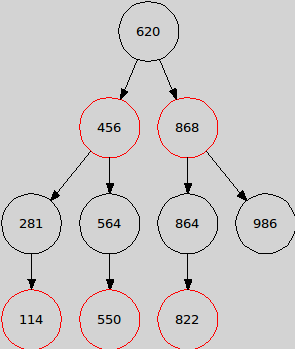
\includegraphics[scale=0.70]{./rbt.png}
\else
\fi
\caption{Red Black Tree}
\label{fig:1}
\end{center}
\end{figure}

The time complexity for insertion and deletion of the nodes are shown in figure 2.  The insertions are done randomly and deletions are done recursively at the root rather than choosing a random node.
\begin{figure}[htb]
\begin{center}
\ifpdf
	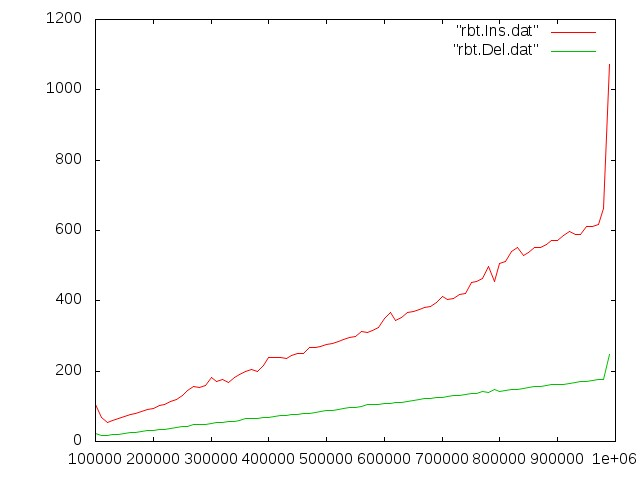
\includegraphics[scale=0.70]{./rbt.jpeg}
\else
%	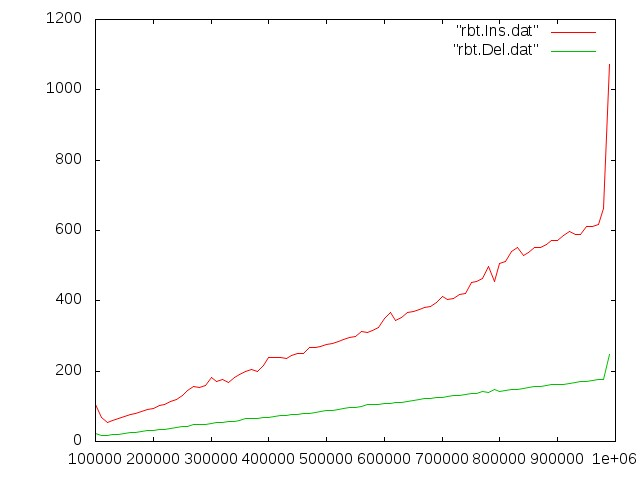
\includegraphics[scale=0.50]{./rbt.jpeg}
\fi
\caption{Red Black Tree: Insertion vs Deletion}
\label{fig:2}
\end{center}
\end{figure}

\newpage 
\begin{thebibliography}{10}
\bibitem{} Cormen, Thomas H et al, 2005, \emph{Introduction to Algorithms---Second Edition}, Prentice-Hall of India.
\end{thebibliography}

\end{document}